\documentclass[11pt,twocolumn]{article}
\usepackage{fontspec}
\usepackage{xeCJK}
\setmonofont{DejaVu Sans Mono}
\usepackage{xcolor}
\definecolor{darkblue}{rgb}{0,0,0.5}
\usepackage[colorlinks=true,allcolors=darkblue]{hyperref}
\usepackage{amsmath}
\usepackage{amssymb}
\usepackage{booktabs}
\usepackage{enumitem}
\setlist{noitemsep}
\usepackage{caption}
\usepackage{subcaption}
\usepackage{sidecap}
\sidecaptionvpos{figure}{c}
\usepackage{graphicx}
\usepackage[sorting=ynt,style=authoryear,uniquename=false]{biblatex}
\addbibresource{paper.bib}
\usepackage{appendix}
\usepackage{fancyvrb}
\usepackage{tikz-cd}
\usetikzlibrary{decorations.pathmorphing}
\DeclareMathOperator{\softmax}{softmax}
\DeclareMathOperator{\relu}{relu}

\title{Sentence simplification with character-level transformer}
\author{%
  Kuan Yu \qquad Sonu Rauniyar \qquad Maya Angelova \qquad Philipp Schoneville\\
  \textit{\{kuanyu, rauniyar, schoneville\}@uni-potsdam.de}\\
  \textit{maya.angelova@protonmail.com}\\
  \\
  Master's Program in \emph{Cognitive Systems}\\
  University of Potsdam}
\date{September 2018}

\begin{document}
\maketitle

\begin{abstract}
  We applied the transformer,
  a neural network architecture developed for machine translation,
  to the task of sentence simplification.
  We modeled sentences at the character level,
  using automatically aligned sentence pairs from the English Wikipedia and the Simple English Wikipedia.
  Our system demonstrated text normalization capacities but only elementary simplification abilities,
  due to the limitations of the data.
  However we made effectual revisions to the transformer,
  and learned various lessons from our explorations.
\end{abstract}

\section{Introduction}

Text simplification can be formulated as translation from a language into a sublanguage
with reduced linguistic complexities,
and the task can be automated using machine translation systems
\parencite{wubben2012sentence, narayan2014hybrid, xu2016optimizing}.
Such systems must know the distributional properties of the source and the target languages,
and model a mapping which preserves the semantic and discourse structures.

Machine translation systems commonly model sentences at the word level.
However, due to the Zipfian distribution of words in a natural language,
the vocabulary can never be fully modeled.
In order to handle unknown words,
it is common practice to replace the low frequency ones in the data with one special symbol.
Among the rare words are proper names and large numbers,
information which should be preserved during translation,
therefore a word-level system needs to be augmented with components for named entity recognition and placement,
along with the component for tokenization.
Additional components inevitably introduce errors and instabilities.
In comparison, a character-level system can be more robust and just as effective \parencite{kalchbrenner2016neural}.
Sophisticated hybrid systems have also been proposed \parencite{luong2016achieving, wu2016google}.
Ideally, such a model learns the morphology to construct new words,
which makes it easier applicable to more languages such as agglutinative ones.
Our system models sentences on the character level.

The transformer is a neural network architecture developed for machine translation
with great success \parencite{vaswani2017attention}.
The architecture relies on attention layers,
as opposed to the conventional recurrent and convolutional layers.
It has since been used for constituency parsing \parencite{kitaev2018constituency},
language generation \parencite{liu2018generating},
image generation \parencite{parmar2018image},
and speech recognition \parencite{zhou2018syllable, zhou2018multilingual}.
The goal of our project is to apply the transformer for sentence simplification.

We made effectual revisions to the transformer in our open source implementation.%
\footnote{\tiny\url{https://github.com/srewai/explicharr}}
Our system demonstrated text normalization capacities and elementary simplification abilities.
In this paper we first describe the background of the machine learning model
(Section~\ref{sec:background}), with a focus on attention mechanisms.
Then we discuss the experiment setup (Section~\ref{sec:setup}),
specifically the data and the evaluation criteria,
and explain our revised architecture (Section~\ref{sec:architecture}).
Finally we describe the training process and examine the results (Section~\ref{sec:results}),
and present our conclusion (Section~\ref{sec:conclusion}).

\section{Background}%
\label{sec:background}

\subsection{Encoder-decoder}

\begin{figure}
  \centering
  \begin{tikzcd}
    T^{\ast}_{0} \ar[bend left]{r} \ar[bend right]{rr} \ar[bend left]{rrr} &T^{\ast}_{1} \ar[bend right]{r} \ar[bend left]{rr} &T^{\ast}_{2} \ar[bend left]{r} &T^{\ast}_{3}\\
  \end{tikzcd}
  \caption[]{\label{fig:autoreg}An autoregressive network.}
\end{figure}

Sequence-to-sequence neural networks are a popular choice for learning text simplification
\parencite{wang2016experimental, zhang2017constrained, vu2018sentence}.
A sequence-to-sequence network usually consists of an encoder and a decoder,
trained jointly with pairs of sequences.
The encoder learns a representation for the source sequences,
and the decoder learns to reconstruct the target sequences from the representation.
Since these sequences vary in their lengths,
a multi-layer perceptron (MLP) is not the ideal architecture,
while recurrent networks are well-suited \parencite{sutskever2014sequence},
and a convolutional one can be effective as well \parencite{gehring2017convolutional}.

The decoder is often autoregressive,
which means that it constructs a sequence one step at a time,
conditioning on the previous steps,
as shown in Figure~\ref{fig:autoreg}.
Here it also has to globally condition on the outputs from the encoder.
Formally, a sequence-to-sequence encoder-decoder models the mapping
\(\forall i \in \mathbb{N}, \left(S^{\ast}, T^{\ast}_{0 \ldots i}\right) \to T^{\ast}_{i+1}\),
where \(S^{\ast}\) are the collection of source sequences freely generated by the collection of source symbols \(S\),
and \(T^{\ast}\) the target sequences generated by \(T\).
Since each target step may have arbitrarily many dependencies from the previous target steps
as well as the source steps,
a good mechanism is needed to determine the importance of these dependencies
and to combine them into a single representation.
Attention is one such choice.

\subsection{Attention mechanisms}

\begin{figure*}
  \begin{subfigure}{0.5\textwidth}
    \centering
    \begin{tikzcd}
      &\hat{x}_{1} &\hat{x}_{2} &\hat{x}_{3}\\
      &\bullet{} \ar[violet]{u} &\bullet{} \ar[violet]{u} &\bullet{} \ar[violet]{u}\\
      &x_{0} \ar[red, bend left]{u} \ar[blue]{u} \ar[blue]{ur} \ar[blue]{urr} &x_{1} \ar[red, bend left]{u} \ar[blue]{u} \ar[blue]{ur} \ar[blue]{ul} &x_{2} \ar[red, bend left]{u} \ar[blue]{u} \ar[blue]{ul} \ar[blue]{ull}\\
    \end{tikzcd}
    \caption*{Encoder self-attention}
  \end{subfigure}%
  \begin{subfigure}{0.5\textwidth}
    \centering
    \begin{tikzcd}
      &\hat{x}_{1} &\hat{x}_{2} &\hat{x}_{3}\\
      &\bullet{} \ar[violet]{u} &\bullet{} \ar[violet]{u} &\bullet{} \ar[violet]{u}\\
      &x_{0} \ar[red, bend left]{u} \ar[blue]{u} \ar[blue]{ur} \ar[blue]{urr} &x_{1} \ar[red, bend left]{u} \ar[blue]{u} \ar[blue]{ur} &x_{2} \ar[red, bend left]{u} \ar[blue]{u}\\
    \end{tikzcd}
    \caption*{Decoder self-attention}
  \end{subfigure}
  \caption[]{\label{fig:layer}Self-attention layers.
    Arrows of the same color denotes linear transformations with the same parameters.
    The red arrows produce the queries,
    the blue arrows produce the values and keys,
    and the black bullets are the attention cells
    which produce the summaries.
    The purple arrows produce the outputs,
    which may be part of the next layer.}
\end{figure*}

A general description for the commonly used soft attention is as follows,
given a query vector and multiple value vectors:

\begin{enumerate}
  \item The query determines a scalar weight for each value;
  \item The weights are then normalized to a probability distribution over the values, typically with
    the \(\softmax\)\footnote{\(\softmax : \mathbb{R}^{n} \to \mathbb{R}^{n},
      x_{i} \mapsto \exp x_{i} / \sum_{j=1}^{n}{\exp x_{j}}\)} function;
  \item The summary is simply the weighted sum of the values.
\end{enumerate}

\textcite{bahdanau2014neural} introduced an attention mechanism to machine translation known as additive attention,
typically used in a recurrent structure.
The recurrent state is used as query.
Each value vector is concatenated with the query and passed into an MLP to produce the attention weight.
The usual choice for the MLP has a single hidden layer with \(\tanh\) activation.
\textcite{luong2015effective} introduced another mechanism where the attention weight is simply
the dot product between the query and the value.
This is known as dot-product or multiplicative attention.
\textcite{daniluk2017frustratingly} introduced key-value attention,
where the value vectors are split into two parts, the values and the keys.
Only the key vectors are used with the query to produce the weights.
This separates the tasks for the model to learn good representations for the values and the keys.

One common application of attention is for the decoder to attend to the encoder outputs,
but it can also be used for both the encoder and the decoder to attend to its own data
without any recurrent structure \parencite{parikh2016decomposable}.
This is known as self-attention or intra-attention.
In sequence learning, self-attention means that a query is simply one time step among the sequence,
and the values are the whole sequence or a subsequence.
The summarized value becomes an annotated representation for data at the time step queried,
with contextual knowledge of all data within the attended time steps.
Due to the autoregressive nature of the decoder,
it must not attend to the future steps.
Figure~\ref{fig:layer} illustrates the self-attention layers.

\begin{figure*}
  \begin{subfigure}{0.5\textwidth}
    \centering
    \begin{tikzcd}
      &\hat{x}_{1} &\hat{x}_{2} &\hat{x}_{3}\\
      &+ \ar[violet]{u} &+ \ar[violet]{u} &+ \ar[violet]{u}\\
      \ar[red]{ur} &x_{0} \ar[blue]{u} \ar[red]{ur} &x_{1} \ar[blue]{u} \ar[red]{ur} &x_{2} \ar[blue]{u}\\
    \end{tikzcd}
    \caption*{Convolutional}
  \end{subfigure}%
  \begin{subfigure}{0.5\textwidth}
    \centering
    \begin{tikzcd}
      &\hat{x}_{1} &\hat{x}_{2} &\hat{x}_{3}\\
      \ar[red]{r} &\bullet{} \ar[violet]{u} \ar[red]{r} &\bullet{} \ar[violet]{u} \ar[red]{r} &\bullet{} \ar[violet]{u}\\
      &x_{0} \ar[blue]{u} &x_{1} \ar[blue]{u} &x_{2} \ar[blue]{u}\\
    \end{tikzcd}
    \caption*{Recurrent}
  \end{subfigure}
  \caption[]{\label{fig:conv-rec}A convolutional layer with filter size 2 and stride 1,
    and a recurrent layer where the black bullets denote the recurrent cell,
    cf. Figure~\ref{fig:layer}.}
\end{figure*}

For comparison, Figure~\ref{fig:conv-rec} illustrates the more commonly used convolutional and recurrent layers
in the context of sequence learning.
In a convolution layer, each step can only access information from a fixed number of input steps,
but the computations for all input steps are independent and can be parallelized.
In a recurrent layer, the recurrent state carries information from all past steps,
but the sequential nature makes training slow.
The recurrent state may be an information bottleneck due to its fixed size,
and long distance dependencies may be difficult to learn.
While self-attention layers combine the advantages of convolutional layers and recurrent layers,
its computational complexity is quadratic instead of linear with respect to the length of the sequence,
since each step may query every other step.

Without either locality or temporal dependency,
the attention mechanism does not respect the ordering of a sequence.
\textcite{gehring2017convolutional} proposed to add positional information to the data,
in the form of a learned position embedding.
\textcite{vaswani2017attention} proposed to hard-code the positional information as sinusoids.
For dimension \(i\) and position \(j\), the encoding is defined as
\(p(j, 2i) = \sin \left( j / 10000^{2i/d} \right)\) and
\(p(j, 2i+1) = \cos \left( j / 10000^{2i/d} \right)\)
where \(d\) is the total number of dimensions.
The motivation is that the wavelengths form a geometric progression from \(\tau\) to \(10000 \tau\),
and that the relative distance between positions can be expressed as a linear function.
Unlike with a learned position embedding,
the length of sequences are not limited by the maximum position learned.

\subsection{Transformer}

\begin{SCfigure*}[4]
  \centering
  \tikz[overlay]{
    \draw[green] (0.0,-1.25) rectangle (1.0,0.75);
    \draw[green] (2.2,-1.25) rectangle (3.2,1.9);}
  \begin{tikzcd}[column sep=tiny]
    &&\hat{T}^{*}_{1 \ldots i+1}\\
    &&\cdot \ar[violet]{u}\\
    \cdot \ar[blue]{rr} &&\bullet{} \ar[violet, rightsquigarrow]{u}\\
    \bullet{} \ar[violet, rightsquigarrow]{u} &&\bullet{} \ar[red]{u}\\
    + \ar[blue, bend left]{u} \ar[red, bend right]{u} &&+ \ar[blue, bend left]{u} \ar[red, bend right]{u}\\
    S^{*} \ar[violet]{u} &P \ar[dashed]{ul} \ar[dashed]{ur} & T^{*}_{0 \ldots i} \ar[violet]{u}\\
  \end{tikzcd}
  \caption[]{\label{fig:transformer}A transformer
    with the encoder on the left and the decoder on the right.
    \(P\) is the position encoding.\\
    The straight arrows are linear transformations,
    the dashed arrows are identity functions,
    and the squiggly arrows are position-wise MLPs.\\
    The coloring matches the scheme in Figure~\ref{fig:layer}.
    The same color signifies the same interpretation,
    and not (necessarily) the same parameters.\\
    The green boxes mark the transformer layers,
    which can be stacked to increase the depth.\\
    The graph omits the residual connections and layer normalizations after each sublayer.}
\end{SCfigure*}

The transformer uses scaled dot-product attention,
a novel variant of key-value dot-product attention.
The attention weights are divided by the square root of the representation dimension
before normalized by the \(\softmax\) function.
The scaling normalizes the variance of dot products.
On top of that, it introduced multi-head attention.
The query space is split into multiple disjoint subspaces.
Each split is an attention head.
The same is done for the key space and the value space.
For each head, the scaled dot-product attention produces a summary,
and the combined summary is their concatenation,
namely the direct sum of the subspaces.
Since each head decides its own list of attention weights,
the same position can be treated with different importance in different subspaces of its representation.
\textcite{vaswani2017attention} explained the splitting of heads
as projections to subspaces with learned linear transformations.
In order to simplify the interpretation,
we treat these linear transformations as procedures immediately before the attention mechanism,
and the projection maps are reduced to fixed orthogonal projections,
implemented as taking subvectors.

Since the attention mechanism alone merely produces a summary from a linear combination of values,
the transformer also uses position-wise MLPs to increase the depth.
Each MLP consists of two layers with
\(\relu\)\footnote{\(\relu : \mathbb{R} \to \mathbb{R}, x \mapsto \max(0, x)\)} activation between,
applied to each position separately.
Each attention layer or MLP is followed by dropout \parencite{srivastava2014dropout},
residual connection \parencite{he2016deep}, and layer normalization \parencite{ba2016layer}.
They are the sublayers in a transformer layer.
A transformer layer in the encoder consists of a self-attention layer followed by an MLP,
and a decoder layer has a secondary attention layer attending to the encoder outputs
in order to condition the construction of target sequences on the source sequences.
Figure~\ref{fig:transformer} illustrates the full architecture.

\section{Setup}%
\label{sec:setup}

\subsection{Data preparation}
\label{ssec:data}

The Simple English Wikipedia provides abundant data
for training text simplification systems \parencite{napoles2010learning}.
Efforts have been made to align its sentences with the ones in the standard English Wikipedia
\parencite{coster2011simple, hwang2015aligning}.
It has also been argued that the Wikipedia datasets are not ideal for the task
of learning text simplification \parencite{xu2015problems}.
However they remain a popular choice due to the accessibility and the quantity.
In our experiments, we used the automatically aligned sentences classified as good and good partial
by \textcite{hwang2015aligning}.\footnote{\tiny\url{http://ssli.ee.washington.edu/tial/projects/simplification/}}

The Wikipedia data come with a large set of characters,
over two thousand in either the standard or the simple parts.
However the top 256 most frequent ones account for 99.97\% of the character count.
We replaced the rest with the non-breaking whitespace,
and cleaned up a few text normalization errors.
We also removed aligned sentences which are identical or longer than 256 characters,
after which we are left with 226\,208 instances.
We randomly picked 1\% to be used for validation,
and the rest for training.

\subsection{Evaluation}

Machine translation systems are commonly measured by the BLEU score,
a value indicating how similar the outputs are to some reference translations produced by human experts.
In our case, the reference translations are the aligned sentences from the Simple English Wikipedia.
\textcite{vstajner2015deeper} argued that the BLEU score is not a good measure for text simplification systems,
with which we agree.
For our validation data, matching the source sentences against the target sentences yield a high BLEU score of 29.53,
which means that the model simply has to learn an identity function to cheat the metric.
Even though we removed identical sentence pairs,
\textasciitilde{}78\% of the character pairs in the training data are still identical in matching positions.
Learning to replicate the source is indeed an easy strategy for the model.

We did not have a solution to this problem.
In our experiments, we primarily judged the goodness of learning by monitoring the validation loss and accuracy.
As a secondary criterion, we took the BLEU scores and inspected the outputs.
Our baseline model (BLEU = 25.44) was a word-level transformer.

\section{Architecture}%
\label{sec:architecture}

We started with a faithful reimplementation of the original transformer,
but made various changes to the design during our experiments.
In order to explain our design choices,
here is an reexamination for the attention mechanisms.

\subsection{Attention reexamined}

\begin{figure*}
  \begin{subfigure}{0.5\textwidth}
    \centering
    \begin{tikzcd}
      v &&\\
      wt \cdot t \ar[violet]{u}{vw} &t \ar[swap]{l}{\softmax}\\
      vt \ar[blue]{u}{wv} \ar[blue, swap]{r}{kv} &kt + k \ar[rightsquigarrow, swap]{u}{\textrm{MLP}} &q \ar[red]{l}{kq}\\
    \end{tikzcd}
    \caption*{Additive attention}
  \end{subfigure}%
  \begin{subfigure}{0.5\textwidth}
    \centering
    \begin{tikzcd}
      v &&\\
      wt \cdot t \ar[violet]{u}{vw} &&\\
      vt \ar[blue]{u}{wv} \ar[blue, swap]{r}{kv} &kt \cdot^{T} k \ar[swap]{ul}{\softmax} &q \ar[red]{l}{kq}\\
    \end{tikzcd}
    \caption*{Dot-product attention}
  \end{subfigure}
  \caption[]{\label{fig:attention}Attention mechanisms with
    \(t\) time steps, \(q\) query dimensions, \(k\) key dimensions,
    \(v\) value dimensions, and \(w\) intermediate value dimensions.
    For the simplicity of notation,
    we use the shape of an object to denote the object itself.
    To unify matrix multiplication and batched dot product,
    we treated vectors as column matrices,
    and define \(A \cdot B := A B\)
    whereas \(A \cdot^{T} B := A^{T} B\).}
\end{figure*}

Figure~\ref{fig:attention} demonstrates the general forms of additive attention and dot-product attention.
Given a query vector of \(q\) dimensions,
and a sequence of value vectors of \(v\) dimensions and \(t\) time steps,
packed into a value matrix of shape \(vt\),
the attention mechanism produces a summarized value vector of \(v\) dimensions.
Two matrices \(kq\) and \(kv\) performs the linear transformations
from the query space and the value space to the key space,
where the query and values can be matched to produce the attention weights.
Another linear transformation \(wv\) produces the actual values to be weighted.
Finally \(vw\) transforms the summary to a value vector for the next layer.
This process is repeated for each time step.
The interpretation of these linear transformations may vary in specific designs.
For example, with additive attention,
the key transformation \(kv\) is in fact part of the MLP after concatenation,
and the value transformation \(wv\) is usually the identity function,
unless key-value attention is used, in which case it is an orthogonal projection.
Also the final transformation \(vw\) may be part of the next layer.

Additive attention is computationally expensive.
The MLP has to operate on \(kt + k\) for all time steps,
which is a tensor with a shape of batch size times \(kt^{2}\) during training.
In dot-product attention, that tensor is immediately contracted.
Unless we restrict \(k\) to a very small number,
it is not feasible to apply additive attention in a fully attention-based model.
We experimented with \(k = 2, 4, 8, 16\) and found training to be much more difficult than
models with dot-product attention using a similar amount of memory.
The model learned slower per training step and each training step takes much longer.
Therefore we focused our experiments on dot-product attention.

\subsection{Revisions}

\begin{figure}
  \centering
  \begin{tikzcd}
    v &&\\
    vt \cdot t \ar[violet, rightsquigarrow, swap]{u}{\textrm{MLP}} &&\\
    vt \ar[blue, dashed]{u} \ar[blue, dashed]{r} &vt \cdot^{T} v \ar[swap]{ul}{\softmax} &q \ar[red, rightsquigarrow, swap]{l}{\textrm{MLP}}\\
  \end{tikzcd}
  \caption{\label{fig:revis}Revised attention cell, cf. Figure~\ref{fig:attention}.}
\end{figure}

The linear transformation for keys and values are useful
if we wish to set the dimensions \(k\) and \(w\) to be different from \(v\).
However in the our transformer and the original,
all dimensions (\(q\), \(k\), \(v\), and \(w\)) are kept the same.
We observed that in dot-product attention,
the key transformation \(kv\) is in fact redundant.
By replacing \(kq\) with \(kv \cdot^{T} kq\) and \(kv\) with identity,
the resulting attention weights would remain the same.
Hence the model could simply learn the key transformation, if it is necessary at all,
as part of the query transformation.
Similarly, the value transformation \(wv\) is also redundant.
The model could simply learn \(vw\) as \(vw \cdot wv\),
due to the associativity of linear transformations.

Since the dot product is a bilinear form,
and both the key and the query transformations are linear,
the original dot-product attention can only model bilinear maps,
whereas the additive attention uses an MLP which is
a universal function approximator \parencite{hornik1989multilayer}.
\textcite{vaswani2017attention} observed that additive attention outperforms dot-product attention
for large representation dimensions while for small dimensions they perform similarly,
which motivated the proposed scaling factor.
We used an MLP for the query transformation.
While the attention weights are still linear with the value space,
the resulting summary is no longer a simple linear combination of values.
This is important for the self-attention layers,
where the query comes from the same space as the values.

Figure~\ref{fig:revis} illustrates our revised dot-product attention.
These changes expand the modeling capacity of the attention layers
without increasing the computational complexity.
In fact, omitting the key and value transformations makes dynamic caching easier.
When running the decoder autoregressively,
the transformation for one time step is needed for all future steps.
Caching the keys and values is necessary to avoid repeating the same computation.
However, the query transformation is always new to the current step.
Therefore having only the query transformation means only the results after each layer need to be cached.
This problem can be understood by counting the number of connections in Figure~\ref{fig:layer}.

\subsection{Multi-head or single-head}

After replacing the linear query transformation with an MLP,
we found that the multi-head design was no longer beneficial,
judging from the validation loss and accuracy.
We hypothesize that the real benefits of multi-head attention was due to the combination of two factors:
The \(\softmax\) function used for weight normalization,
and the linear transformation used for the query.
The \(\softmax\) function normalizes the exponentiated dot products by the \(l_{1}\) norm.
During exponentiation, the large positive weights are inflated,
exaggerating the importance of the corresponding values over all the other values,
which likely causes a winner-take-all situation.
Having multiple attention heads mitigates this problem,
while having an MLP to transform the query offers the same flexibility.

To test this hypothesis, we tried squaring instead of exponentiating the dot products.
We found that with linear query transformations,
the training dynamics of single-head attention by squaring was similar to
multi-head attention with \(\softmax\), which were both notably better than single-head attention with \(\softmax\).
With MLPs for query, single-head attention learned faster than multi-head,
and it was more stable with \(\softmax\) than with squaring.

Although these findings supports our hypothesis,
we believe the true efficacy of multi-head attention still needs to be investigate in a setup
with a metric of success more meaningful than the validation loss and accuracy we used for this task.
However we did consistently find scaling helpful for \(\softmax\).
Note that in the case of normalized squares, scaling simply has no mathematical effect.
In summary, we decided on single-head attention with \(\softmax\) and scaling.

\subsection{Final architecture}

\begin{figure}
  \centering
  \tikz[overlay]{
    \draw[green] (0.0,-1.25) rectangle (1.0,0.75);
    \draw[green] (2.2,-1.25) rectangle (3.2,1.9);}
  \begin{tikzcd}[column sep=tiny]
    &&\hat{T}^{*}_{1 \ldots i+1}\\
    &&\cdot \ar[violet]{u}\\
    \cdot \ar[blue, dashed]{rr} &&\bullet{} \ar[violet, rightsquigarrow]{u}\\
    \bullet{} \ar[violet, rightsquigarrow]{u} &&\bullet{} \ar[red, rightsquigarrow]{u}\\
    + \ar[blue, dashed, bend left]{u} \ar[red, rightsquigarrow, bend right]{u} &&+ \ar[blue, dashed, bend left]{u} \ar[red, rightsquigarrow, bend right]{u}\\
    S^{*} \ar[violet]{u} &P \ar[dashed]{ul} \ar[dashed]{ur} & T^{*}_{0 \ldots i} \ar[violet]{u}\\
  \end{tikzcd}
  \caption[]{\label{fig:arch}Revised transformer, cf. Figure~\ref{fig:transformer}.}
\end{figure}

Figure~\ref{fig:arch} illustrates our revised transformer architecture.
We used two encoder layers and two decoder layers.
The dimension of hidden representations was 256 throughout the model,
except for the inner \(\relu\) layer of the MLPs,
which was doubled to 512.
This was adopted from the original transformer,
where the inner dimensions were quadrupled but with no explanation given.
We found that having a larger inner layer was effective in preventing the dying \(\relu\) problem,
where all neurons in a layer were updated to always produce zero activation during training
which would render the whole model useless and unable to recover.

We experimented with input and output embedding sharing \parencite{press2016using},
which was used in the original transformer.
It seemed to hurt the training dynamics of our character-level model,
where these embedding layers had only a moderate amount of parameters.
We also did not enforce parameter sharing between the two input embeddings.

\section{Training and results}%
\label{sec:results}

\subsection{Training}

Autoregressive networks with temporal updates are commonly trained using teacher forcing,
a technique derived from the maximum likelihood criterion \parencite{williams1989learning}.
Instead of feeding the outputs of the model back to itself to train for the next time step,
the ground truth values are used as inputs.
This way, the training for all time steps can take place in parallel.
The attention weights can be computed for all steps against every other step simultaneously,
both in the encoder and the decoder.
However in the decoder, the upper triangle of the self-attention weight matrix has to be masked out
in order to maintain the autoregressive structure.
This is done by setting the unnormalized weights to \(- \infty\) \parencite{vaswani2017attention}.

We discovered that masking is also necessary for the source sequences.
In batched training, all sequences in one batch are padded to the same length.
Ideally the model would learn to ignore the paddings,
but we observed that this was not what happens.
The trained model behaved differently when fed the same sequence with different numbers of paddings.
Therefore we masked the padding positions for all attention layers.

Our training scheme is almost identical to the original transformer.
The training objective is to minimize the cross entropy between the predictions
and the ground truth targets with a smoothing rate of 0.1 \parencite{szegedy2016rethinking}.
We used the Adam optimizer \parencite{kingma2014adam} with
\(\beta_{1} = 0.9, \beta_{2} = 0.98, \varepsilon = 10^{-9}\)
and a learning rate
\(d^{-0.5} \min \left(s^{-0.5}, w^{-1.5}s\right)\)
where \(s\) is the training step,
\(d = 256\) the model dimension,
and \(w = 4000\) the number of warmup steps.
We also used a dropout rate of 0.1,
but we did not apply dropout to the position encoding.
We found that the model took much longer to reach the same validation loss and accuracy
when the position encoding was dropped out,
and it did not improve the results in the long run.
We tried the time-sharing dropout scheme suggested for recurrent networks
by \textcite{gal2016theoretically},
but it did not seem to suit the transformer.

We experimented with other training schemes.
With teacher forcing, the decoder only receives ground truth sequences during training,
which might differ significantly from the autoregressively generated sequences
which it depends on for inference.
Therefore we tried training the model with free-running inputs.
We ran the model autoregressively to produce a sequence,
and used that sequence as the input to predict the truth sequence.
We mixed the training schedule with teacher forcing.
It was expected that the predictions would worsen in free-running mode,
but in the long run, the model should become more robust.
However that was not what we found.
Free-running training always worsened the model,
even when evaluated in teacher forcing mode.

We also tried training with backpropagation through time (BPTT).
Since the softmax outputs describe the predicted distribution for the next character,
we can multiply the probabilities with the embedding matrix for a weighted representation of the next input,
and the computation for all steps can be chained for backpropagation.
Training with BPTT is slow and expensive in memory usage,
but it was also ineffective.
The accumulation of uncertainty caused the prediction to degrade over time.
the highest probability started from \textasciitilde{}60\% and dropped to \textasciitilde{}15\%.
the second highest stayed \textasciitilde{}10\%.
When the highest prediction dropped below 20\%,
the model would simply repeat a character, usually the whitespace.

As a result, we committed to teacher forcing training.
We used a batch size of 64, and trained the model for 180 epochs.
The training speed was \textasciitilde{}10 iterations per second on a graphics card.
One significant drawback of modeling at the character level is that the sequences are much longer.
We suspected that it would be difficult to apply the transformer architecture to long sequences,
due to its quadratic complexity with lengths.
However thanks to its high parallelizability,
it is still efficient for our task.

\subsection{Results}

We used eager decoding for the autoregressive model.
The predicted character with the highest probability was taken as the next input.
It produced a BLEU score of 29.59 on the validation set.
Over 80\% of the output sentences were identical to the source.

The model performs some basic text normalization.
It replaces unknown characters with the non-breaking whitespace (\ref{app:1}{1},~\ref{app:2}{2}),
adds or removes brackets for balancing (\ref{app:2}{2},~\ref{app:3}{3}),
and has its own preferences for the format of punctuations (\ref{app:4}{4})
and dates (\ref{app:5}{5}).

Some source sentences are incomplete.
The model always produces normal-looking sentences with initial capitalization and terminal punctuations.
This sometimes reduces the incomplete sentence to a noun phrase (\ref{app:6}{6},~\ref{app:7}{7}),
or a trivial sentence (\ref{app:8}{8},~\ref{app:9}{9}).
It tries to make use of existing information,
but the outcome is often unsatisfying (\ref{app:10}{10},~\ref{app:11}{11}).

For simplification, the model tends to remove the initial adverbial of a sentence
(\ref{app:12}{12},~\ref{app:13}{13},~\ref{app:14}{14}),
but not always (\ref{app:15}{15}).
It removes components in the middle of a sentence
which are usually omitted in the Simple English Wikipedia
(\ref{app:16}{16},~\ref{app:17}{17},~\ref{app:18}{18}).
It also removes words with no additional information (\ref{app:19}{19},~\ref{app:20}{20}),
and may add simple words such as particles (\ref{app:21}{21}),
or substitute some words with simpler ones (\ref{app:22}{22}).

On rare occasions, the model behaves erratically (\ref{app:23}{23},~\ref{app:24}{24}).
This happens when the decoding steps lose alignment with the source positions,
as shown in Figure~\ref{fig:align}.

\begin{figure}
  \centering
  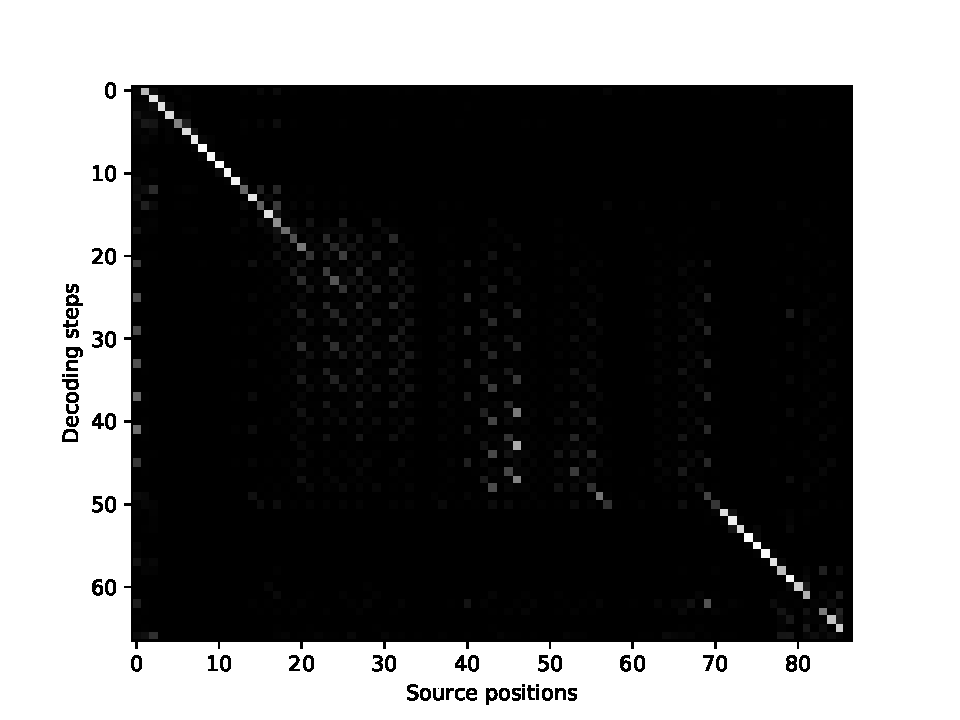
\includegraphics[width=0.5\textwidth,page=1]{plot.pdf}
  \caption[]{\label{fig:align}Attention alignment for example~\ref{app:23}{23}.}
\end{figure}

\section{Conclusion}%
\label{sec:conclusion}

Our model was able to learn the common forms of English sentences,
and the general differences between the two Wikipedias,
as demonstrated by its text normalization capacities.
However as a text simplification system,
its performance is unsatisfying.
It has only limited abilities to simplify whole constituents,
often by deletion.
It shows no ability for syntactic transformations
and no understanding for semantic structures.

Nevertheless, we do not consider our architecture unsuitable for the task.
As shown in Appendix~\ref{sec:app},
many aligned sentence pairs differ in content.
Even among the pairs which do correspond in content,
the ground truth targets are rarely good simplifications for the sources.
However wherever good examples exist,
the model does produce the same or similar outputs.
We need more suitable examples of sentence simplification with interesting linguistic properties.

\printbibliography[]

\appendix
\onecolumn
\section{Output examples}
\label{sec:app}

Each output example is a triple of sentences:
the source, the prediction, and the ground truth target.
The examples are from the validation set, cf. Section~\ref{ssec:data}.

\subsection*{Example 1}
\label{app:1}
\begin{Verbatim}[fontsize=\scriptsize]
The enshrined kami is Isonotakeru no mikoto ( 五十猛命 ? )

The enshrined kami is Isonotakeru no mikoto (      ? )

This place is special to the kami named Isonotakeru no mikoto ( 五十猛命 ? )
\end{Verbatim}

\subsection*{Example 2}
\label{app:2}
\begin{Verbatim}[fontsize=\scriptsize]
Edo ( 江户 ?

Edo (    ? )

Edo ( 江户 ? )
\end{Verbatim}

\subsection*{Example 3}
\label{app:3}
\begin{Verbatim}[fontsize=\scriptsize]
Buddha-Bhagavan ) .

Buddha-Bhagavan .

Buddhists believe there have been many Buddhas who were alone , called pacceka-buddhas .
\end{Verbatim}

\subsection*{Example 4}
\label{app:4}
\begin{Verbatim}[fontsize=\scriptsize]
Punch 's wife was originally called `` Joan . ''

Punch 's wife was originally called `` Joan '' .

Punch 's wife was originally `` Joan '' .
\end{Verbatim}

\subsection*{Example 5}
\label{app:5}
\begin{Verbatim}[fontsize=\scriptsize]
Their first child , Prince George of Cambridge , was born on 22 July 2013 .

Their first child , Prince George of Cambridge , was born on July 22 , 2013 .

On July 24 , it was announced that the baby would be called Prince George of Cambridge ,
with the full given name George Alexander Louis .
\end{Verbatim}

\subsection*{Example 6}
\label{app:6}
\begin{Verbatim}[fontsize=\scriptsize]
is a 1982 arcade-style platform video game by Nintendo .

In 1982 , the style platform video game by Nintendo .

Donkey Kong Jr. is an arcade video game made by Nintendo in 1982 .
\end{Verbatim}

\subsection*{Example 7}
\label{app:7}
\begin{Verbatim}[fontsize=\scriptsize]
reflects the influence of the sexagenary cycle as a count of years .

The influence of the sexagenary cycle as a count of years .

Ancient records show that the sexagenary cycle was used to count years in the 3rd century B.C. .
\end{Verbatim}

\subsection*{Example 8}
\label{app:8}
\begin{Verbatim}[fontsize=\scriptsize]
and Mario 's Time Machine .

The machine is a machine .

In the Dr. Mario games first seen in 1990 , Mario is a doctor .
\end{Verbatim}

\subsection*{Example 9}
\label{app:9}
\begin{Verbatim}[fontsize=\scriptsize]
and Airplane II : The Sequel .

The Sequel is a sequel .

( 1980 ) and Airplane II : The Sequel ( 1982 ) .
\end{Verbatim}

\subsection*{Example 10}
\label{app:10}
\begin{Verbatim}[fontsize=\scriptsize]
and it is because they do n't understand what Parkour is ; ` Who is the best ? '

They are the best ?

Star Jumping Parkour does involve risks and many people get injured every day .
\end{Verbatim}

\subsection*{Example 11}
\label{app:11}
\begin{Verbatim}[fontsize=\scriptsize]
It is officially known as Avtomat Kalashnikova ( Russian : Автомат Калашникова ) .

It is known as Avtomat Kalashnikova ( Russian : : 1950 : 1998 ) .

The letters AK stand for Avtomat Kalashnikova , which is Russian for Kalashnikov 's Automatic Rifle .
\end{Verbatim}

\subsection*{Example 12}
\label{app:12}
\begin{Verbatim}[fontsize=\scriptsize]
With one huge blow from his olive-wood club , Hercules killed the watchdog .

Hercules killed the watchdog .

Herakles killed her .
\end{Verbatim}

\subsection*{Example 13}
\label{app:13}
\begin{Verbatim}[fontsize=\scriptsize]
For example , the speed of sound in gases depends on temperature .

The speed of sound in gases depends on temperature .

Loudness depends on sound intensity , sound frequency , and the person 's hearing .
\end{Verbatim}

\subsection*{Example 14}
\label{app:14}
\begin{Verbatim}[fontsize=\scriptsize]
In it , Goldilocks is re-imagined as a girl in her 20s .

Goldilocks is re-imagined as a girl in her 20s .

She finally became Goldilocks sometime in the early 20th century .
\end{Verbatim}

\subsection*{Example 15}
\label{app:15}
\begin{Verbatim}[fontsize=\scriptsize]
In 2008 , she starred in the comedy film Baby Mama , alongside former SNL co-star Amy Poehler .

In 2008 , she starred in the comedy movie Baby Mama , alongside former SNL co-star Amy Poehler .

In 2008 , she starred in the comedy movie Baby Mama , with Amy Poehler .
\end{Verbatim}

\subsection*{Example 16}
\label{app:16}
\begin{Verbatim}[fontsize=\scriptsize]
The spines , which may be up to 50 mm ( 2 in ) long , are modified hairs , mostly made of keratin .

The spines , which may be up to 50 mm long , are modified hairs , mostly made of keratin .

The spines , which may be up to 50 mm long , are modified hairs , mostly made of keratin .
\end{Verbatim}

\subsection*{Example 17}
\label{app:17}
\begin{Verbatim}[fontsize=\scriptsize]
Sodium iodate ( NaIO3 ) is the sodium salt of iodic acid .

Sodium iodate is the sodium salt of iodic acid .

Sodium iodate is a chemical compound .
\end{Verbatim}

\subsection*{Example 18}
\label{app:18}
\begin{Verbatim}[fontsize=\scriptsize]
The palate / ˈpælɨt / is the roof of the mouth in humans and other mammals .

The palate is the roof of the mouth in humans and other mammals .

The palate is the roof of the mouth in humans and other mammals .
\end{Verbatim}

\subsection*{Example 19}
\label{app:19}
\begin{Verbatim}[fontsize=\scriptsize]
It is located in the Market Square , Aylesbury , Buckinghamshire .

It is in the Market Square , Aylesbury , Buckinghamshire .

The King 's Head is a National Trust property in Aylesbury , Buckinghamshire , England , UK .
\end{Verbatim}

\subsection*{Example 20}
\label{app:20}
\begin{Verbatim}[fontsize=\scriptsize]
Home Alone received mixed reviews from film critics .

Home Alone received mixed reviews from critics .

Home Alone 3 ( 1997 ) and Home Alone 5 : The Holiday Heist ( 2012 )
have completely different characters and actors .
\end{Verbatim}

\subsection*{Example 21}
\label{app:21}
\begin{Verbatim}[fontsize=\scriptsize]
However , low frequency also causes noticeable flicker in arc lamps and incandescent light bulbs .

The low frequency also causes noticeable flicker in arc lamps and incandescent light bulbs .

This happens so fast that a light bulb does not stop glowing .
\end{Verbatim}

\subsection*{Example 22}
\label{app:22}
\begin{Verbatim}[fontsize=\scriptsize]
In the film 's story the location was named as Footscray station .

In the movie 's story the location was named as Footscray station .

In the movie it was called Footscray station .
\end{Verbatim}

\subsection*{Example 23}
\label{app:23}
\begin{Verbatim}[fontsize=\scriptsize]
For example , 2 + 3 = 3 + 2 = 5 and 2 · 3 = 3 · 2 = 6 , but 23 = 8 , whereas 32 = 9 .

For example , 2 + 3 = 3 = 3 = 3 = 3 = 3 = 3 = 3 , whereas 32 = 9 .

Then people write powers using the ^ sign : 2 ^ 3 means .
\end{Verbatim}

\subsection*{Example 24}
\label{app:24}
\begin{Verbatim}[fontsize=\scriptsize]
1 and − 1 divide ( are divisors of ) every integer .

In the 19th century , the state of the state of the state of the state of the state of the state
of the state .

For example , if the last digit is even ( 0 , 2 , 4 , 6 or 8 ) , then 2 is a divisor .
\end{Verbatim}

\end{document}
